\documentclass[11pt,]{book}
\usepackage{lmodern}
\usepackage{setspace}
\setstretch{2}
\usepackage{amssymb,amsmath}
\usepackage{ifxetex,ifluatex}
\usepackage{fixltx2e} % provides \textsubscript
\ifnum 0\ifxetex 1\fi\ifluatex 1\fi=0 % if pdftex
  \usepackage[T1]{fontenc}
  \usepackage[utf8]{inputenc}
\else % if luatex or xelatex
  \ifxetex
    \usepackage{mathspec}
  \else
    \usepackage{fontspec}
  \fi
  \defaultfontfeatures{Ligatures=TeX,Scale=MatchLowercase}
\fi
% use upquote if available, for straight quotes in verbatim environments
\IfFileExists{upquote.sty}{\usepackage{upquote}}{}
% use microtype if available
\IfFileExists{microtype.sty}{%
\usepackage{microtype}
\UseMicrotypeSet[protrusion]{basicmath} % disable protrusion for tt fonts
}{}
\usepackage[margin=1in]{geometry}
\usepackage{hyperref}
\hypersetup{unicode=true,
            pdfborder={0 0 0},
            breaklinks=true}
\urlstyle{same}  % don't use monospace font for urls
\usepackage{natbib}
\bibliographystyle{apalike}
\usepackage{longtable,booktabs}
\usepackage{graphicx,grffile}
\makeatletter
\def\maxwidth{\ifdim\Gin@nat@width>\linewidth\linewidth\else\Gin@nat@width\fi}
\def\maxheight{\ifdim\Gin@nat@height>\textheight\textheight\else\Gin@nat@height\fi}
\makeatother
% Scale images if necessary, so that they will not overflow the page
% margins by default, and it is still possible to overwrite the defaults
% using explicit options in \includegraphics[width, height, ...]{}
\setkeys{Gin}{width=\maxwidth,height=\maxheight,keepaspectratio}
\IfFileExists{parskip.sty}{%
\usepackage{parskip}
}{% else
\setlength{\parindent}{0pt}
\setlength{\parskip}{6pt plus 2pt minus 1pt}
}
\setlength{\emergencystretch}{3em}  % prevent overfull lines
\providecommand{\tightlist}{%
  \setlength{\itemsep}{0pt}\setlength{\parskip}{0pt}}
\setcounter{secnumdepth}{5}
% Redefines (sub)paragraphs to behave more like sections
\ifx\paragraph\undefined\else
\let\oldparagraph\paragraph
\renewcommand{\paragraph}[1]{\oldparagraph{#1}\mbox{}}
\fi
\ifx\subparagraph\undefined\else
\let\oldsubparagraph\subparagraph
\renewcommand{\subparagraph}[1]{\oldsubparagraph{#1}\mbox{}}
\fi

%%% Use protect on footnotes to avoid problems with footnotes in titles
\let\rmarkdownfootnote\footnote%
\def\footnote{\protect\rmarkdownfootnote}

%%% Change title format to be more compact
\usepackage{titling}

% Create subtitle command for use in maketitle
\newcommand{\subtitle}[1]{
  \posttitle{
    \begin{center}\large#1\end{center}
    }
}

\setlength{\droptitle}{-2em}
  \title{}
  \pretitle{\vspace{\droptitle}}
  \posttitle{}
  \author{}
  \preauthor{}\postauthor{}
  \date{}
  \predate{}\postdate{}

\usepackage{booktabs}
\usepackage{amsthm}
\usepackage[utf8]{inputenc}
\usepackage[english]{babel}
\makeatletter
\def\thm@space@setup{%
  \thm@preskip=8pt plus 2pt minus 4pt
  \thm@postskip=\thm@preskip
}
\makeatother

\addcontentsline{toc}{chapter}{\listtablename}{ix}
\addcontentsline{toc}{chapter}{\listfigurename}{xi}

\begin{document}

\begin{center}
\begin{titlepage}
\bf{The Pennsylvania State University} \\
The Graduate School \\
College of Medicine Public Health Sciences \\

STATISTICAL MODELS FOR HIGH DIMENSIONAL SCREENING OF GENETIC AND EPIGENETIC EFFECTS

A Dissertation in \\
Biostatistics \\
by \\
Kirk Gosik \\
(c) 2017 Kirk Gosik \\

Doctor of Philosophy \\
February 2017 \\
\end{titlepage}
\newpage
\pagenumbering{roman}
\setcounter{page}{2}
The dissertation of Kirk Gosik was reviewed and approved* by the following:

Rongling Wu \\
Distinguished Professor of Public Health Sciences and Statistics \\
Thesis Advisor, Chair of Committee

Vernon Chinchilli \\
Distinguished Professor and Chair of Public Health Sciences


Lan Kong \\
Associate Professor of Public Health Sciences

James Broach \\
Distinguished Professor and Chair of Biochemistry and Molecular Biology \\


\newpage

Abstract

Knowledge about how changes in gene expression are encoded by expression quantitative trait loci (eQTLs) is a key to construct the genotype-phenotype map for complex traits or diseases. Traditional eQTL mapping is to associate one transcript with a single marker at a time, thereby limiting our inference about a complete picture of the genetic architecture of gene expression. Here, I present innovative applications of variable selection approaches to systematically detect main effects and interaction effects among all possible loci on differentiation and function of gene expression and other phenotypes of interest. Forward-selection-based procedures were particularly implemented to tackle complex covariance structures of gene-gene interactions. Simulation studies were performed on each of the models to assess the computational properties of each model.  Applications of the models were also performed on real datasets.  The first was a reanalysis of a published genetic and genomic dataset collected in a mapping population of Caenorhabditis elegans, gaining new discoveries on the genetic origin of gene expression differentiation, which could not be detected by a traditional one-locus/one-transcript analysis approach.  The next dataset was of Mei Tree growth, analyzing the genetic control of the height and diameter during the developmental process.  The underlying genotypes and epistasis that impact the process of these developments were considered as candidates for the selection of the procedure.

\end{center}

{
\setcounter{tocdepth}{1}
\tableofcontents
}
\listoftables
\listoffigures
\chapter{automatically create a bib database for R
packages}\label{automatically-create-a-bib-database-for-r-packages}

\chapter{Introduction}\label{intro}

\pagenumbering{arabic} \setcounter{page}{1}

\section{Background}\label{background}

There are several techniques used for studying genetics and mapping the
results. Some of the more popular techniques include cross-breeding
experiments or, in the case of humans, the examination of family
histories, known as pedigrees. More recently, CRISPR/Cas9 can be used to
mimic mitotic recombination to help map out genes as well.
(\cite{sadhu2016crispr})

Construction of genetic maps are a variety of techniques used to show
relative positions between genes or other sequence features of the
genome and the phenotype that is controlled by such sequences. Genes are
very useful markers but they are by no means ideal. One problem,
especially with larger genomes such as those of vertebrates and
flowering plants, is that a map based entirely on genes is not very
detailed.(\cite{brown2006genomes}) Genes have long areas of non-coding
regions between them and therefore result in large gaps from gene to
gene. This is further complicated because not every gene has allelic
forms that can be easily or conveniently distinguished. With these
considerations in mind gene maps may not be comprehensive enough and
other markers may be needed.

According to brown, mapped features that are not genes are called DNA
markers. As with gene markers, a DNA marker must have at least two
alleles to be useful. There are three types of DNA sequence feature that
satisfy this requirement: restriction fragment length polymorphisms
(RFLPs), simple sequence length polymorphisms (SSLPs), and single
nucleotide polymorphisms (SNPs). (\cite{brown2006genomes}) The genetic
markers that have been emphasized in this work are single nucleotide
polymorphisms. Attempting to be at the highest levels of resolution for
identifying quantitative traits, using SNPs are the most specific case.
This will give exact location of the nucleotide that may be impacting
the genetic control over the phenotype.

\begin{figure}

{\centering 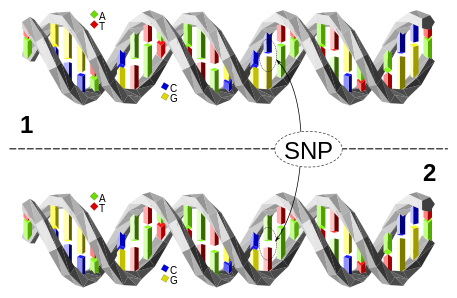
\includegraphics[width=0.8\linewidth]{images/SNP_Picture} 

}

\caption{SNP Picture}\label{fig:Snp-Pic}
\end{figure}

There are several goals to genetic mapping and association studies that
identify certain regions of the genome that contain genes involved in
specifying a quantitative trait, referred to as quantitative trait loci
(QTLs). One main goal is to estimate the genetic effects of these loci.
The relationship between the genetic effects of QTLs and the phenotypic
value of quantitative traits can be described by a linear model
(\cite{collard2005introduction}, \cite{xu2007empirical}). Typically,
because of the high throughput nature of the data there are a large
number of markers across the whole genome, and most of the markers may
have very little or next no effect on the phenotype under study. The
models can be very sparse, with most cases, the number of genetic
markers or variables is bigger than the sample size, especially when
interactions among markers are considered. This makes a model is over
saturated and further model selection techniques may be required to
capture the necessary information. \cite{dong2015accurate}

\begin{figure}

{\centering 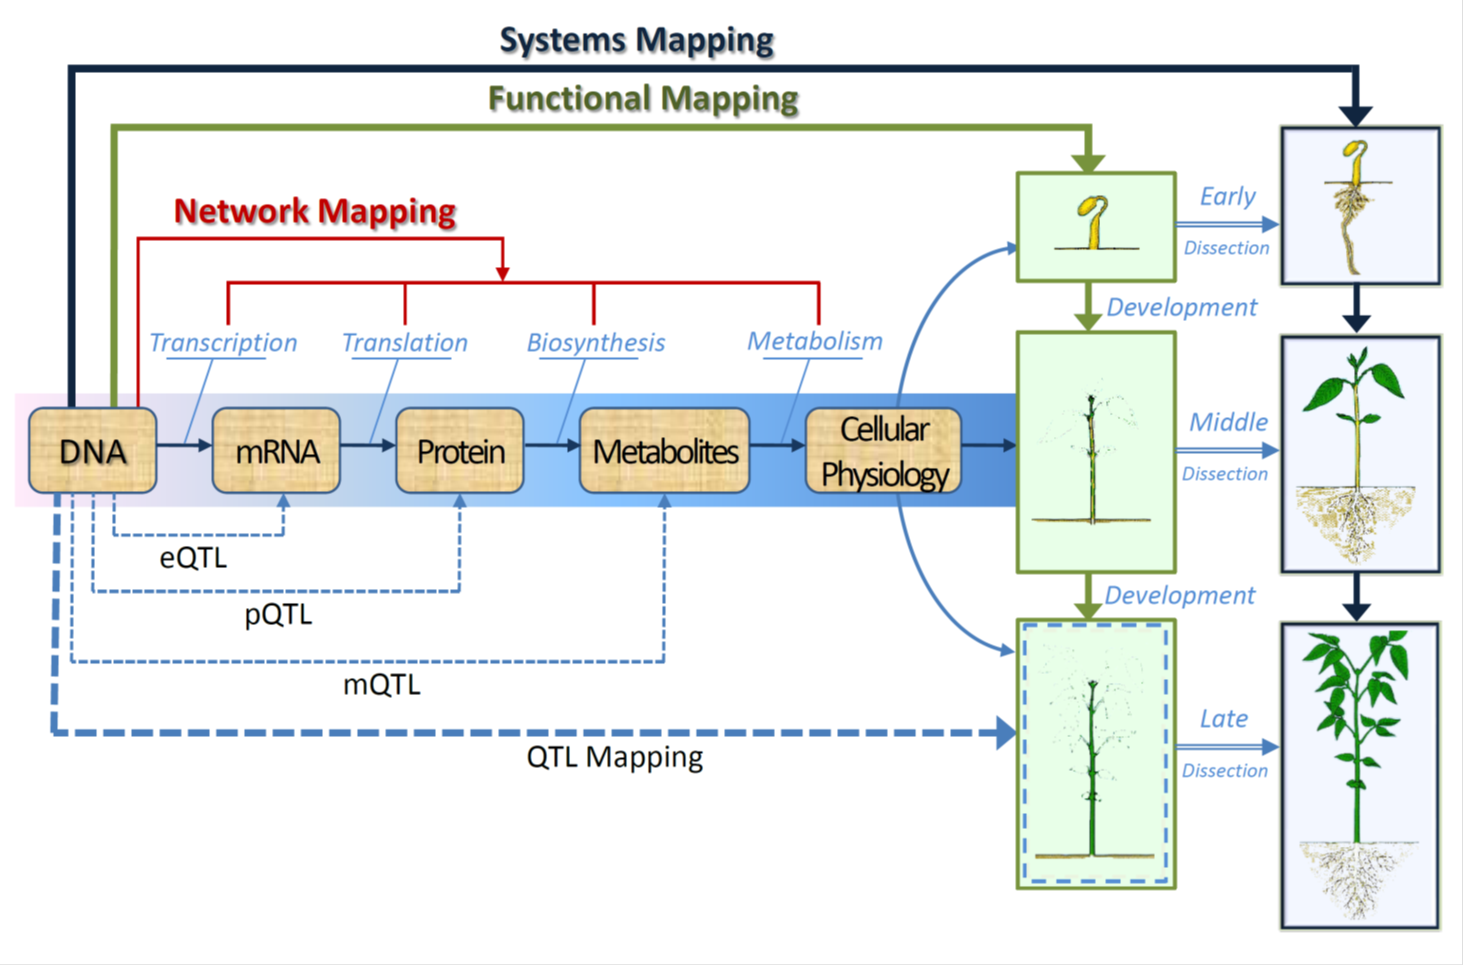
\includegraphics[width=0.8\linewidth]{images/SystemsMapping} 

}

\caption{Systems Map}\label{fig:system-map}
\end{figure}

\section{Some Exisiting Methods}\label{some-exisiting-methods}

Numerous methods exist and are being developed to measure and find
quantitative trait loci (QTL) effects. These methods can broadly fall
into three main categories. These categories are Least-Square methods,
maximum likelihood and Bayesian approaches. (\cite{wu2007statistical})
Each method has advantages and considerations that you would need to be
aware before conducting analyses to find QTL effects from the given
markers. A brief discussions on a few of the methods are given to
highlight some areas of consideration and how the methods proposed can
handle such considerations.

Marker Regression would fall in the category of Least Squares
approaches. If looking at one marker analysis general t-test and ANOVA
procedures can be used to analyze the relationship. It is not
recommended however for use in general practice because you do not know
how dense the markers are measured. QTL interval mapping would be
preferred in such an analysis because the methods take account for
missing genotype data that may not have been measured. When estimating a
QTL position through maximum likelihood methods, like interval mapping,
positions of other possible QTLs could affect the detection of the true
position. Neighboring QTLs could possibly flatten the likelihood in
instances where there are multiple QTLs on the same chromosome. This
would make an effect look less significant at a given location than it
actually is. Another possibility is that in the search over the interval
you may find an area where the likelihood could reach a peak but could
be a ``ghost'' QTL. This is where an effect is observed because a
neighboring QTL is skewing the results at the particular position you
are looking in and the result is a false discovery of the position.
Marker Regression has been shown to improve interval mapping, which is
call Composite Interval Mapping. This is where the QTL position found is
also combined in a linear regression where the covariates are the other
markers in the dataset. By including the markers as covariates the other
position in the chromosome are accounted for in the analysis and false
discovery is reduced.

The analysis of interval mapping and single marker analyses has shown to
be effective but it limits our inference to one marker at a time as a
possible loci that controls a trait. Using Marker Regression however you
can incorporate multiple markers in a single analysis to test for
possible QTL for a given trait. It is cautioned that running such an
analysis is only an approximate test because the null hypothesis is
there is no difference between the marker levels and therefore a
non-mixture distribution but the alternative is a mixture of
distributions. The assumptions regression would make of the errors
within the marker type to be normally distributed may not be entirely
met if the QTL's fall between the marker regions. However
\cite{whittaker1996mapping} have shown that a direct regression of
phenotypes on marker types, provides the same information about location
of QTL-effects without having to step to all positions on the interval.
With this information using the entire marker set in a regression
analysis would provide a nice, computationally efficient way to map out
the genetic architecture of a trait.

\section{Chapter Overview}\label{chapter-overview}

The main theme of this paper is to propose an improvements on selection
procedures which use regression techniques to approach high dimensional
variable selection such as the ones arising in epistatic analysis. The
variable selection procedure for QTL mapping can be seen as one of
deciding which subset of variables have effects on the phenotypes of
interest, and identifying those specific traits out of all possible
effects between the markers. Each procedure proposed is a forward
selecting method that starts with the empty set. After starting with the
empty set each procedure continues to add markers to the model set as
possible QTLs. Once a designated stopping criteria is met the final
model is fit and the effects are estimated. Each of the next three
chapters focuses on a new selection procedure and the properties of
them.

\subsection{HighDeQTL}\label{highdeqtl}

In this chapter we introduce the iform procedure, originally proposed by
(\cite{hao2014interaction}). Included in the chapter is the algorithm
and how it compares to forward selection. From there it is adapted to
use for a genetic mapping studies. The properties of this will be
explored in detail. Simulation studies were conducted to assess how well
the properties are met and under what conditions. Comparisons to other
models was also explored to get a sense of the utility and advantages
that come with the new selection procedure. After the comparisons and
simulations a real world application is performed. The application was a
reanalysis of a data set using C Elegans first proposed by
\cite{rockman2010selection}.

\subsection{Higher Order Epistasis}\label{higher-order-epistasis}

The next chapter considers higher order epistasis and its importance.
Currently it is under studied because of practical limitations not
because of biological limitations or relevance. The iFORM procedure
proposed in Chapter 2 is then extended to incorporate higher orders of
epistatic effects. Even though similar methods are being used the
properties are still studied and assessed. Simulation studies were
performed to assess practical applications. Several scenarios and
comparison models were considered to extensively look at what properties
were being met and which were not. Then an application to Mei tree
growth was conducted in order to see the real world application of such
a selection procedure. Different growth parameters were previously fit
and these were used as the phenotype. Interesting and more predictive
implications came out of the model when considering higher order
epistasis throughout the selection procedure.

\subsection{iForm Funcional Mapping}\label{iform-funcional-mapping}

The application of the Mei tree growth led into exploring to use a more
functional phenotype as a response throughout the selection procedure.
In order to use all relevant information of the repeated measure data,
it would take an additional computation burden to the selection and the
modeling but it would also give more power and flexibility to the
modeling that would not be present otherwise. It is important to use all
relevant information in order to make the most accurate prediction about
the data. Using a growth curve model to assist in fitting the data would
help ease some of the computational burden. The selection of genetic
effects however would be very simplistic as some additive shift to the
curve. This view may not be the most accurate and therefore more
complicated structures will be implemented to produce better results.
Legendre orthogonal polynomials were considered to model the genetic
effects. These polynomials have various forms and would allow for the
genetic effect to follow different patterns but also not induce
unnecessary correlation between predictors when included in the model.
Again, simulation studies were conducted and a reanalysis of the full
Mei tree dataset was considered.

\subsection{Conclusions}\label{conclusions}

Finally in the last chapter it will focus on comparisons and discussion
around the models proposed. Future aims of the research goals will be
explored also. Seeing how my current research will lead into the aims
and what possible directions can be explored with the given statistical
frameworks.

\chapter{High Dimensional eQTL}\label{highdeqtl}

\chapter{High-order Epistatic Networks}\label{highorder}

\chapter{iForm Functional Mapping}\label{iformfunc}

\chapter{Conclusions}\label{conclusions-1}

\chapter{Appendix}\label{appendix}

\chapter{Placeholder}\label{placeholder}

\bibliography{packages.bib,book.bib}
\addcontentsline{toc}{chapter}{\bibname}


\end{document}
